\documentclass[aspectratio=169,14pt,dvipsnames]{beamer}

\title[Refactoring ALICE Masterclasses]{A new framework for the ALICE-Masterclasses}
\author[Jonas Toth, CERN Summer Student]{Jonas Toth \linebreak CERN Summer Student}
\date{23. August 2018}

\usepackage[english]{babel}
\usepackage[utf8]{inputenc}
\setbeamertemplate{footline}[page number]
\setbeamertemplate{blocks}[rounded]
\setbeamerfont{caption}{size=\big}
\beamertemplatenavigationsymbolsempty

%AMSLaTeX packages
\usepackage{minted}
\usepackage{amsmath}
\usepackage{amsfonts}
\usepackage{textcomp}
\usepackage{tikz}
\usepackage{rotating}
\usepackage{transparent}% http://ctan.org/pkg/transparent
\setbeamercovered{transparent}
\newcommand{\hidecontent}[2][0.25]{{% \hidecontent[<transparency>]{<stuff>}
  \setbox9=\hbox{#2}% Store <stuff> in \box9 to obtain height/width
\transparent{#1}\ooalign{\usebox9\cr\color{white}\rule{\wd9}{\ht9}\cr}}}
\usetheme{default}
\useoutertheme{infolines}
\setbeamertemplate{headline}{}
\usepackage{graphicx}
\usepackage[dvips]{epsfig}
\usepackage{dcolumn}
\usepackage[point,rounding]{rccol}
\usepackage{booktabs}
\usepackage{varwidth}
\usepackage{colortbl}
\usepackage{color}
\definecolor{maroon1}{rgb}{1.000000,0.203922,0.701961}
\definecolor{highlightcolor}{RGB}{0,102,204}
\newcommand{\highl}[1]     {\textcolor{highlightcolor}{#1}}
\newcommand{\redmark}[1]     {\textcolor{Maroon}{#1}}
\newcommand{\greenmark}[1]     {\textcolor{OliveGreen}{#1}}
\usepackage[pscoord]{eso-pic}% The zero point of the coordinate systemis the lower left corner of the page (the default).
% \definecolor{darkred}{rgb}{0.8,0.3,0.1}
\usepackage{mathrsfs}
\renewcommand{\thefootnote}{}
\renewcommand{\thefootnote}{\arabic{footnote}}
\renewcommand{\footnoterule}{}
\newcommand{\pT}{$p_{\mbox{\tiny T}}$\xspace}
\newcommand{\pTm}{p_{\mbox{\tiny T}}}
\newcommand{\placetextbox}[3]{% \placetextbox{<horizontal pos>}{<vertical pos>}{<stuff>}
  \setbox0=\hbox{#3}% Put <stuff> in a box
  \AddToShipoutPictureFG*{% Add <stuff> to current page foreground
    \put(\LenToUnit{#1\paperwidth},\LenToUnit{#2\paperheight}){\vtop{{\null}\makebox[0pt][c]{#3}}}%
  }%
}%
\begin{document}
% \setbeamercovered{transparent}
\begin{frame}
  \titlepage
  \vspace{-0.7cm}
  \begin{figure}
    \centering
    
\includegraphics[height=0.3\textheight]{2012-Jul-04-4_Color_Logo_CB.png}\hspace{0cm}
  \end{figure}
\end{frame}

\begin{frame}{
\includegraphics[height=0.07\textheight]{2012-Jul-04-4_Color_Logo_CB.png} \hspace{0.2cm}\textbf{Motivation and Goal}}
  \begin{itemize}
    \item<1> \textbf{Increase public outreach}
    \item<1> deploy everywhere
    \item<1> if possible translate to local language

    \item<2> \textbf{more ALICE MasterClasses in one package}
    \item<2> Strangeness
    \item<2> Raa
    \item<2> J/Psi

    \item<3> \textbf{Allow other experiments and institutes to join}
    \item<4> \textbf{address classical software topics}
  \end{itemize}
\end{frame}

\begin{frame}{
\includegraphics[height=0.07\textheight]{2012-Jul-04-4_Color_Logo_CB.png} \hspace{0.2cm}\textbf{Starting point}}
  \begin{itemize}
    \item Version from Christian Holm Christensen
    \item Repository on \textbf{gitlab.cern.ch}
      % TODO \item Screenshot of initial window (Class and Language Selection)
    \item Macro-based solution with Strangeness and Raa Classes
    \item initial translation facilities
  \end{itemize}
\end{frame}

\begin{frame}{
\includegraphics[height=0.07\textheight]{2012-Jul-04-4_Color_Logo_CB.png} \hspace{0.2cm}\textbf{Starting point}}
  \begin{figure}
    \centering
    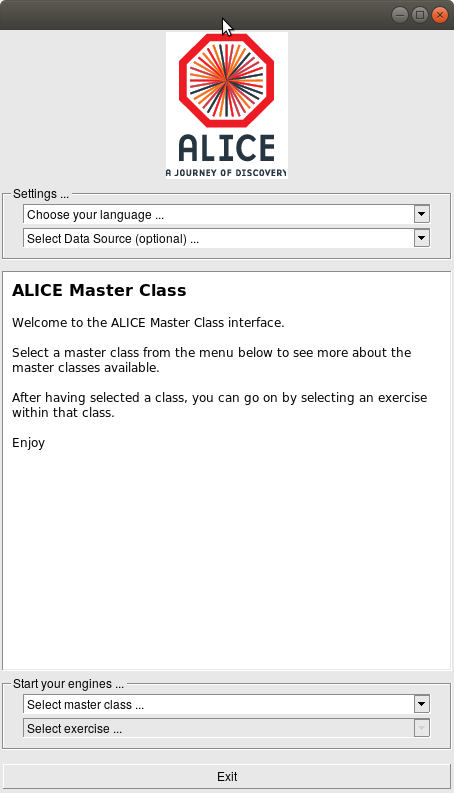
\includegraphics[height=0.8\textheight]{SelectionWindow.png}\hspace{0cm}
  \end{figure}
\end{frame}

\begin{frame}{
\includegraphics[height=0.07\textheight]{2012-Jul-04-4_Color_Logo_CB.png} \hspace{0.2cm}\textbf{New: Full Translation}}
  \begin{itemize}
    \item<1> \textbf{Provide a way to easily add a new language}
    \item<1>\textbf{translate whole program}
    \item<2> added German translation, Dutch is WIP
    \item<2> file-based solution does not require programming skills
    \item<2> static analysis for consistency
    \item<2> semi-automatic snippet translation through Google Translate
    \item<3> \textbf{Groups are encouraged to add translations}
  \end{itemize}
\end{frame}

\begin{frame}[fragile]{
\includegraphics[height=0.07\textheight]{2012-Jul-04-4_Color_Logo_CB.png} \hspace{0.2cm}\textbf{New: Full Translation}}
  \begin{minted}[
      fontsize=\footnotesize,
    ]{c++}
    /// translation/EntryPoint/Description.en.html
    R"(
    <html>
    <head>
    </head>
    <body>
    <h1>ALICE Master Class</h1>

    <p> Content of the user-facing document. Shortened... </p>
    </body>
    </html>)"
  \end{minted}
\end{frame}

\begin{frame}[fragile]{
\includegraphics[height=0.07\textheight]{2012-Jul-04-4_Color_Logo_CB.png} \hspace{0.2cm}\textbf{New: Full Translation}}
  \begin{minted}[
      fontsize=\footnotesize,
    ]{c++}
    /// translation/EntryPoint/keys_gui_trans.txt.en

    /// Key-Value store for English.
    /// every language will define its own set of strings.
    RegisterText("GUISettings", "Settings ...");
    RegisterText("GUIDataSource", "Select Data Source (optional) ...");
    RegisterText("GUILabelClassConfig", "Start your engines ...");
    RegisterText("GUIChooseLanguage", "Choose your language ...");
    RegisterText("GUIChooseClass", "Select master class ...");
    RegisterText("GUIChooseExercise", "Select exercise ...");
    RegisterText("GUIExitButton", "Exit");
  \end{minted}
\end{frame}


\begin{frame}[fragile]{
\includegraphics[height=0.07\textheight]{2012-Jul-04-4_Color_Logo_CB.png} \hspace{0.2cm}\textbf{New: Full Translation}}
  \begin{minted}[
      fontsize=\footnotesize,
    ]{c++}
    /// src/EntryPoint/GUITranslation.h
    /// Provide a class that will provide all available strings
    /// in English.
    struct TGUIEnglish : Utility::TLanguageProvider {
      TGUIEnglish(Utility::ESupportedLanguages lang = Utility::English)
        : TLanguageProvider(lang) {
          /// Registering a Key-Value store for
        /// small strings that are translated
        std::cerr << "Registering English  GUI Selection\n";
        #include "EntryPoint/keys_gui_trans.txt.en"
        /// Statically compile in whole translated HTML files.
        RegisterText("Description",
        #include "EntryPoint/Description.en.html"
        );
      }
    };
  \end{minted}
\end{frame}

\begin{frame}[fragile]{
\includegraphics[height=0.07\textheight]{2012-Jul-04-4_Color_Logo_CB.png} \hspace{0.2cm}\textbf{New: Full Translation}}
  \begin{minted}[
      fontsize=\footnotesize,
    ]{c++}
    /// src/EntryPoint/GUITranslation.h
    /// Makes the strings available as methods.
    /// This ensures on compile-time that only existing strings are
    /// used and avoids common errors like typos in the Key-Value-Access.
    struct TGUIEnglish : Utility::TLanguageProvider {
      TGUIEnglish(Utility::ESupportedLanguages lang = Utility::English);
      /// Create all Methods to request the corresponding text snippets.
      LANG_KEY(GUISettings)
      LANG_KEY(GUIDataSource)
      LANG_KEY(GUILabelClassConfig)
      LANG_KEY(GUIChooseLanguage)
      LANG_KEY(GUIChooseClass)
      LANG_KEY(GUIChooseExercise)
      LANG_KEY(Description)
      LANG_KEY(GUIExitButton)
    };
  \end{minted}
\end{frame}

\begin{frame}[fragile]{
\includegraphics[height=0.07\textheight]{2012-Jul-04-4_Color_Logo_CB.png} \hspace{0.2cm}\textbf{New: Full Translation}}
  \begin{minted}[
      fontsize=\footnotesize,
    ]{c++}
    /// src/EntryPoint/GUITranslation.h
    /// Adding another translation in code is very easy.
    /// The 'LANG_TRANSLATION' macro creates a new class that inherits
    /// all methods from the English pendant and only replaces the
    /// string registrations.
    LANG_TRANSLATION(TGUI, German)
    {
      std::cerr << "Registering German GUI Selection - EntryPoint\n";
      #include "EntryPoint/keys_gui_trans.txt.de"

      RegisterText("Description",
      #include "EntryPoint/Description.de.html"
      );
    }
  \end{minted}
\end{frame}

\begin{frame}{
\includegraphics[height=0.07\textheight]{2012-Jul-04-4_Color_Logo_CB.png} \hspace{0.2cm}\textbf{New: Full Translation}}
  \begin{figure}
    \centering
    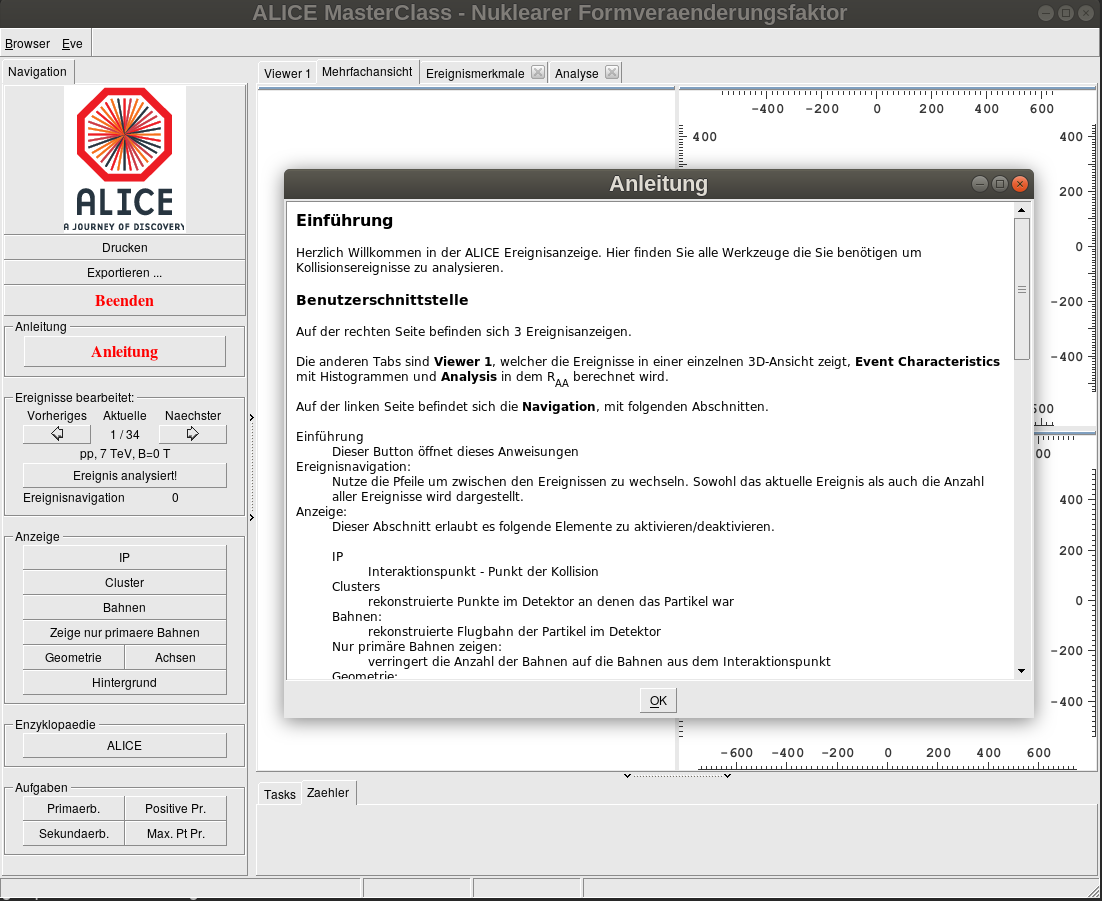
\includegraphics[height=0.8\textheight]{GermanRaa.png}\hspace{0cm}
  \end{figure}
\end{frame}

\begin{frame}{
\includegraphics[height=0.07\textheight]{2012-Jul-04-4_Color_Logo_CB.png} \hspace{0.2cm}\textbf{Refactoring}}
  \begin{block}{Refactoring}
    Structural Changes of Code without affecting behaviour.
  \end{block}

  \begin{itemize}
    \item<2> Missing tests can not catch random breakage
    \item<2> To refactor you need to test, to add tests you need to refactor.
    \item<2> \textbf{Obstacle} every masterclass was copy\&pasted
  \end{itemize}
  % TODO UML Diagram to show, simplified
\end{frame}

\begin{frame}{
\includegraphics[height=0.07\textheight]{2012-Jul-04-4_Color_Logo_CB.png} \hspace{0.2cm}\textbf{Refactor to what?}}
  \begin{block}{SOLID Principles}
    \begin{itemize}
      \item Single Responsibility Principle
      \item Open/Closed Principle
      \item Liskov Substitution Principle
      \item Interface Segregation Principle
      \item Dependency Inversion Principle
    \end{itemize}
  \end{block}
\end{frame}

\begin{frame}[fragile]{
\includegraphics[height=0.07\textheight]{2012-Jul-04-4_Color_Logo_CB.png} \hspace{0.2cm}\textbf{What we want}}
  \begin{minted}[
      fontsize=\footnotesize,
    ]{c++}
    /// Collect statistics over all events in the dataset.
    class TRaaStatistics
    {
      public:
      void AddEventStatistics(const gsl::span<TEveTrack* const> Primaries);
      void AddSecondaryMultiplicity(Int_t NumberSecondaries);
      void ClearStatistics();

      const TH1D& HistMultiplicity() const { return fMultiplicityHist; }
      const TH1D& HistMultiplicityMinPt() const { return fMultHistMinPt; }
      const TH1D& HistMultiplicitySecondaries() const { return fMultHistSec; }
      const TH1D& HistPt() const { return fPtHist; }
      const TH1D& HistCharge() const { return fChargeHist; }
      const TH1D& HistPhi() const { return fPhiDist; }
    };
  \end{minted}
\end{frame}

\begin{frame}[fragile]{
\includegraphics[height=0.07\textheight]{2012-Jul-04-4_Color_Logo_CB.png} \hspace{0.2cm}\textbf{What we don't want}}
  \begin{minted}[
      fontsize=\footnotesize,
    ]{c++}
    /// Just the public interface, a lot more coupling happens through
    /// implicitly shared state.
    class Counter : public TGMainFrame
    {
      public:
      Bool_t fEnableCharge;
      Bool_t fAllowAuto;
      Double_t fHighestPt;
      TEveTrack* fHPtTrack;
      Int_t fSecondaries;
      Counter(const TGWindow* p, UInt_t w, UInt_t h,
              ECollisionSystem collSys, TTrackAnalysis* hists,
              Bool_t allowAuto = false);
      TGNumberEntryField* AddField(TGCompositeFrame* cf, TGLayoutHints* lh,
                                   Bool_t isInt = false, Bool_t neg = false);
      void Build();
      /// ...
  \end{minted}
\end{frame}


\begin{frame}[fragile]{
\includegraphics[height=0.07\textheight]{2012-Jul-04-4_Color_Logo_CB.png} \hspace{0.2cm}\textbf{What we don't want}}
  \begin{minted}[
      fontsize=\footnotesize,
    ]{c++}
      /// ...
      void Reset(ECollisionSystem collSys, Bool_t ResetAll = true);
      void DoExit() { this->UnmapWindow(); }
      void CountAutomatic();
      void Reset(Bool_t ResetAll = true);
      void Instructions();
      void Fill(Double_t px, Double_t py, Double_t pz, Int_t charge);
      void IncreaseMult(Double_t pt);
      void Publish();
      void FillHistAuto(Double_t pt, Double_t q, TEveTrack* track,
                        Double_t phi);
      /// End of interface
    };
  \end{minted}
\end{frame}

\begin{frame}{
\includegraphics[height=0.07\textheight]{2012-Jul-04-4_Color_Logo_CB.png} \hspace{0.2cm}\textbf{Extend Raa-Class}}
  \begin{itemize}
    \item<1-> criticism was a too monotonic experience when selecting only primary tracks
    \item<2-> Implement four tasks to choose from
    \item<2-> distinguish between primary and secondary particle
    \item<2-> distinguish between charges
    \item<2-> estimate particle momentum from curvature
    \item<3-> \textbf{explore more physics}
  \end{itemize}
  % TODO Add screenshot from new event display
  % TODO Maybe do a demo on this one
\end{frame}

\begin{frame}{
\includegraphics[height=0.07\textheight]{2012-Jul-04-4_Color_Logo_CB.png} \hspace{0.2cm}\textbf{Extend Raa-Class}}
  \begin{figure}
    \centering
    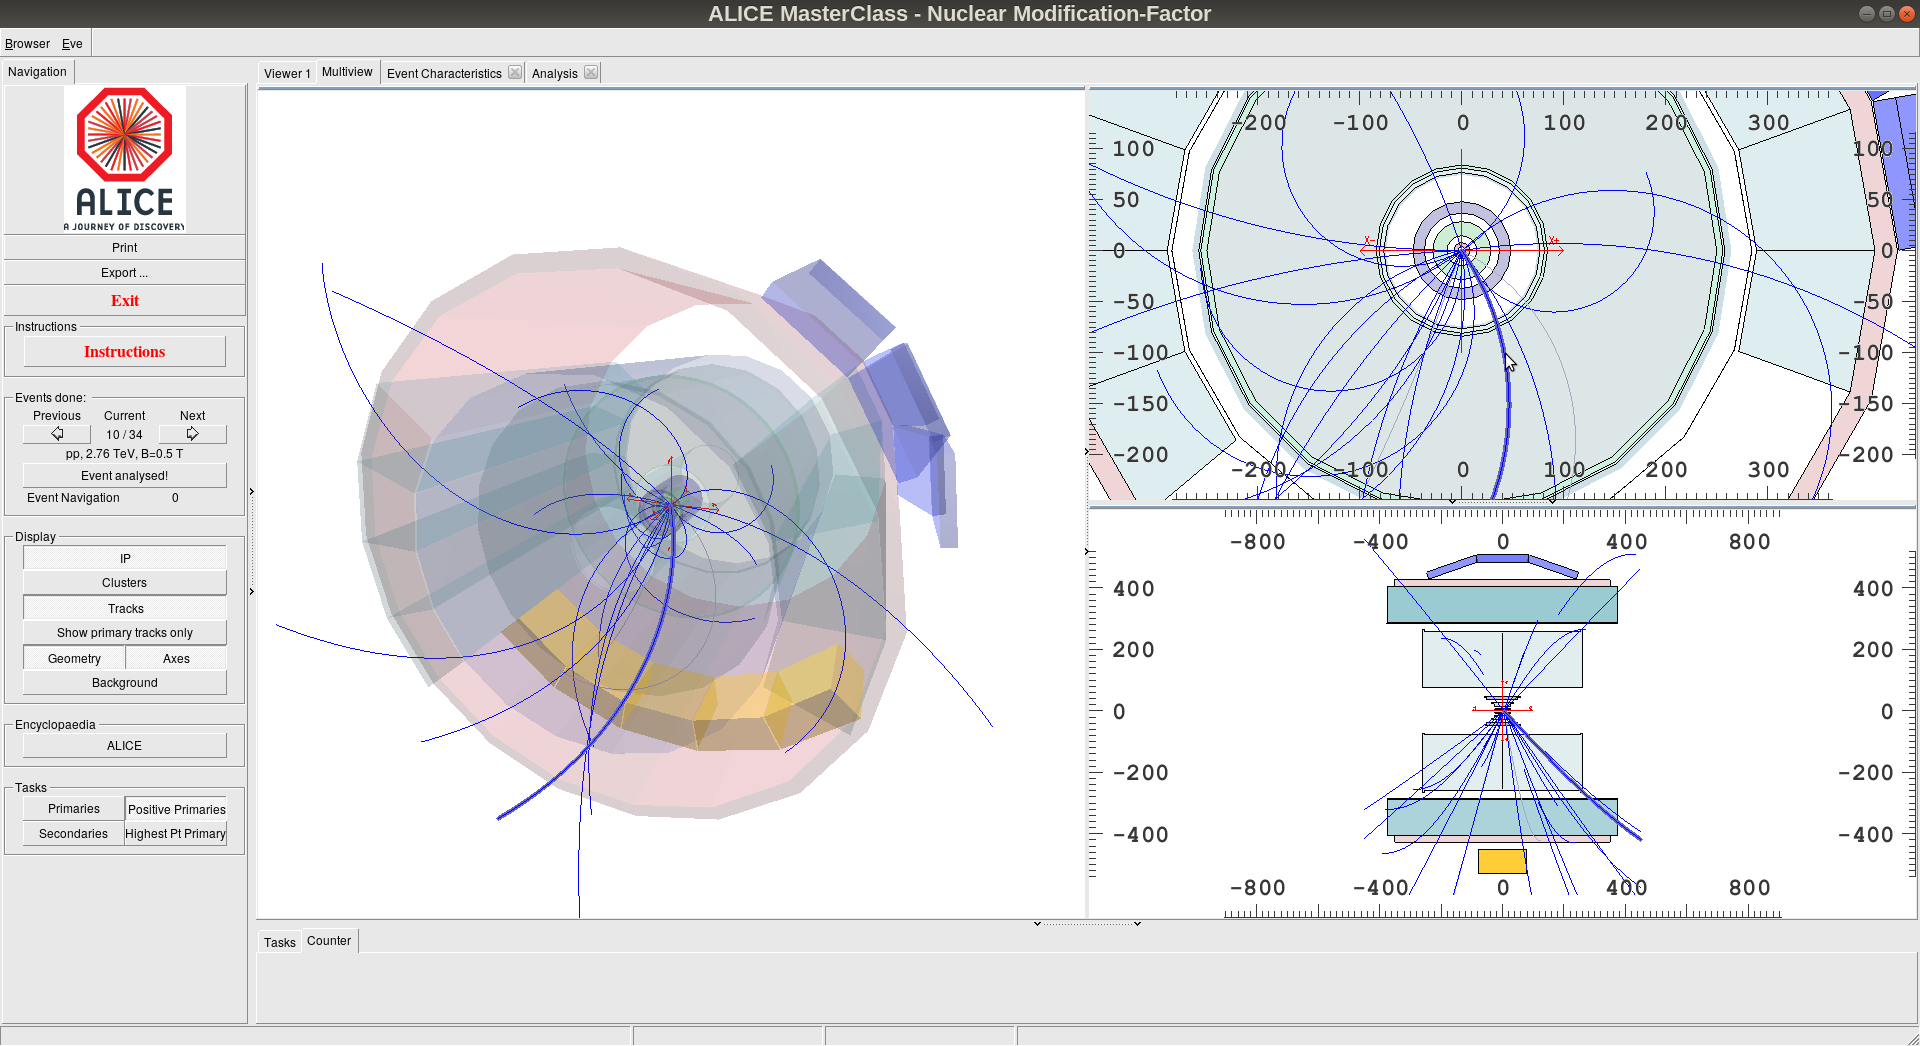
\includegraphics[height=0.8\textheight]{EventDisplayAndTasks.png}\hspace{0cm}
  \end{figure}
\end{frame}

\begin{frame}{
\includegraphics[height=0.07\textheight]{2012-Jul-04-4_Color_Logo_CB.png} \hspace{0.2cm}\textbf{New J/Psi Masterclass}}
  \begin{itemize}
    \item Implemented from GSI
    \item right now just a code dump
      % TODO Make more clear that it already runs
    \item can be run the same way as Strangeness and Raa
  \end{itemize}
\end{frame}

\begin{frame}{
\includegraphics[height=0.07\textheight]{2012-Jul-04-4_Color_Logo_CB.png} \hspace{0.2cm}\textbf{New J/Psi Masterclass}}
  \begin{figure}
    \centering
    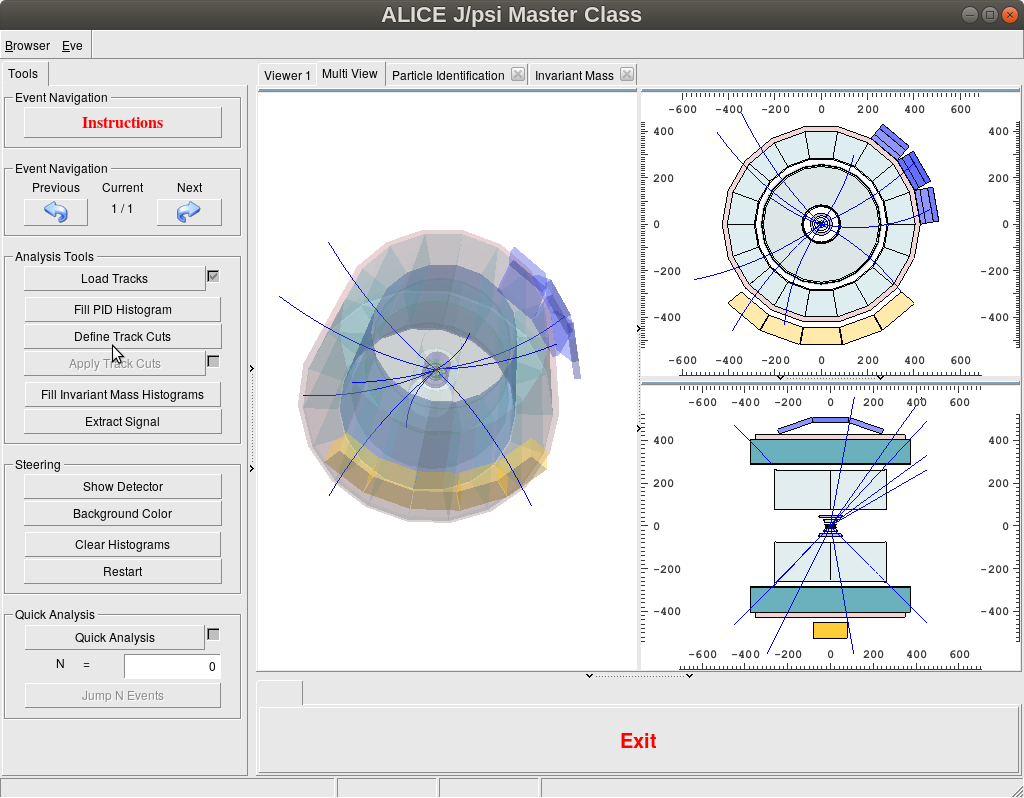
\includegraphics[height=0.8\textheight]{JPsiClass.png}\hspace{0cm}
  \end{figure}
\end{frame}

\begin{frame}{
\includegraphics[height=0.07\textheight]{2012-Jul-04-4_Color_Logo_CB.png} \hspace{0.2cm}\textbf{Deployment and Usage}}
  \begin{itemize}
    \item<1-> ROOT6 to be future proof
    \item<2-> compiled executable (only Linux at the moment)
    \item<2-> requires only ROOT6 installed on the system
    \item<2-> CMake based process
    \item<3-> all masterclasses in one package
    \item<3-> Goal to have Linux AppImage
  \end{itemize}
\end{frame}

\begin{frame}{
\includegraphics[height=0.07\textheight]{2012-Jul-04-4_Color_Logo_CB.png} \hspace{0.2cm}\textbf{Outlook}}
  \begin{itemize}
    \item jsROOT implements Event-Display for browser
    \item \href{https://root.cern.ch/js/latest/?nobrowser\&json=../files/geom/simple_alice.json.gz\&file=../files/geom/tracks_hits.root\&item=simple_alice.json.gz+tracks_hits.root/tracks;1+tracks_hits.root/hits;1}{Link to Example}
    \item Web-based Masterclasses instead of ROOT-GUI
    \item the basic architecture and structure can be reused
    \item WebAssembly, ASM.js and Emscrippten allow code-reuse
  \end{itemize}
\end{frame}

\begin{frame}{
\includegraphics[height=0.07\textheight]{2012-Jul-04-4_Color_Logo_CB.png} \hspace{0.2cm}\textbf{Outlook jsROOT}}
  \begin{figure}
    \centering
    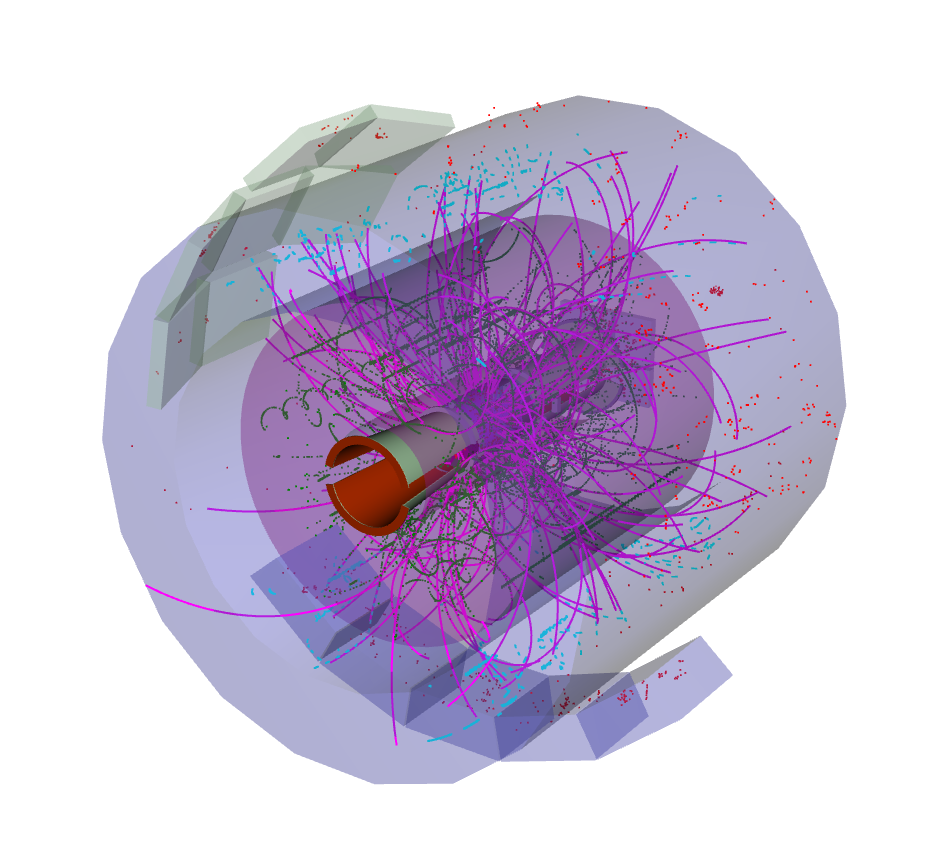
\includegraphics[height=0.8\textheight]{jsROOTDisplay.png}\hspace{0cm}
  \end{figure}
\end{frame}

\begin{frame}[noframenumbering]{}
  \begin{center}
    \textbf{\fontsize{30pt}{10pt}{Questions}}
  \end{center}
\end{frame}

\begin{frame}[noframenumbering]{Finalizing my work}
  \begin{itemize}
    \item automatically generating packages containing everything
    \item start refactoring J/Psi as well
    \item double-check all elements of the masterclasses to detect breakages
  \end{itemize}
\end{frame}

\end{document}
